\section{Anforderungen und Konzeption}
\subsection{Anforderungen}
Dieses Kapitel beschreibt die Anforderungen des Projektes. Das Projekt ist die Implementierung und die Analyse einer Spiel-KI für das Spiel \textit{"Ganz schön clever"}.
\subsubsection{Rahmenbedingungen}
Es ist eine Künstliche Intelligenz zu implementieren, welche das Spiel \textit{"Ganz schön clever"} gut spielen können soll. Dazu muss zunächst die Spielumgebung entwickelt und implementiert werden. Mithilfe dieser soll ein Verfahren entwickelt werden, welches die Künstliche Intelligenz in dieser Umgebung trainieren soll.

Anschließend sind die Ergebnisse des Entwicklungsprozesses sowie des Erzeugnisses selbst zu analysieren und vorzustellen. Dies soll mithilfe geeigneter, schlüssiger sowie verständlicher Methoden und Visualisierungstechniken erfolgen.
\subsubsection{Spiel}
Das Spiel heißt \textit{"Ganz schön clever"}. Ziel des Spiels ist es, möglichst viele Punkte innerhalb einer vorgeschriebenen Rundenanzahl zu erreichen [siehe Unterabschnitt 2.1.1].

Zunächst soll ein Prototyp der Spielumgebung entwickelt werden, welcher später schrittweise erweitert werden soll, bis das Spiel mit allen Funktionalitäten implementiert worden ist.\\

Diese Funktionalitäten sind:
\begin{itemize}
\item Die sechs farbigen Würfel, welche geworfen werden können und zufällig eine Würfelzahl von 1 bis 6 liefern. Es werden dabei immer alle aktuell gültigen Würfel gleichzeitig geworfen.

\item Ein Mechanismus, welcher die Würfel für die aktuelle Runde als ungültig markiert, sobald sie gewählt werden. Ungültige Würfel dürfen nicht gewählt werden [siehe Unterabschnitt 2.1.1].

\item Ein Mechanismus, welcher Würfel mit einer niedrigeren Augenzahl als der aktuell gewählte Würfel als ungültig für die Runde markiert, solange sich das Spiel nicht in einer Wahl vom Silbertablett oder einer Wahl mithilfe des Extra-Wahl-Bonus befindet.

\item Ein Runden-System, bei dem insgesamt sechs Runden gespielt werden, in denen jeweils bis zu drei Würfe erfolgen, solange bei einem der Würfe noch gültige Würfel vorhanden sind. Zudem erfolgt nach jeder Runde die Auswahl eines Würfels vom Silbertablett, welches die ungültigen Würfel eines anderen Spielers beinhaltet. Wenn das Spiel alleine gespielt wird und es dadurch keinen anderen Spieler gibt, werden hierzu alle Würfel geworfen und drei davon auf das Silbertablett gelegt. Außerdem werden Boni am Anfang der ersten, zweiten, dritten und vierten Runde für alle Spieler freigeschaltet [siehe Unterabschnitt 2.1.1].

\item Die fünf farbigen Felder, gelb, blau, grün, orange und lila. Jedes Feld hat seine eigenen Regeln, wenn es darum geht wann ein Würfel gewählt werden darf, um eines der Kästchen auf diesem Feld auszufüllen [siehe Unterabschnitt 2.1.1]. Die Felder beinhalten verschiedene Belohnungen, die freigespielt werden, wenn bestimmte Kästchen oder Kombinationen aus diesen ausgefüllt worden sind [siehe Unterabschnitt 2.1.1].

\item Die zehn verschiedenen Boni, Fuchs, Extra-Wahl, Neu-Würfeln, Gelbes-Kreuz, Blaues-Kreuz, Grünes-Kreuz, Orangene-Vier, Orangene-Fünf, Orangene-Sechs sowie Lila-Sechs [siehe Unterabschnitt 2.1.1]. Dies beinhaltet sowohl das Erhalten, Speichern, sowie die Benutzung der Boni.

\item Ein Mechanismus, welcher Würfel, die mithilfe eines Extra-Wahl-Bonus gewählt wurden, als ungültig markiert, damit diese nicht erneut in der selben Runde durch mit einem Extra-Wahl-Bonus gewählt werden können.

\item Ein Mechanismus, der Würfel zur richtigen Zeit wieder als gültig markiert. Dies erfolgt nach dem dritten Wurf in der Runde, nach Extra-Wahlen im eigenen Zug (nach dem dritten Wurf), nach der Wahl vom Silbertablett des Gegners und nach Extra-Wahlen, die nach der Wahl vom Silbertablett des Gegners erfolgen. Würfel werden nicht nach jedem Einsatz eines Extra-Wahl-Bonus wieder gültig, sondern erst nachdem der Spieler keinen weiteren Extra-Wahl-Bonus mehr hat oder sich entscheidet zum gegebenen Zeitpunkt keinen weiteren zu verwenden.
\end{itemize}
\subsubsection{Künstliche Intelligenz}
Die Künstliche Intelligenz soll das Spiel möglichst gut spielen können. Es sollen geeignete Methoden zur Verfügung stehen, um die KI trainieren und mit ihr nach dem Training Vorhersagen [siehe Unterabschnitt 2.1.2] treffen zu können. Außerdem sollte sie Möglichkeiten bieten verschiedene Parameter anzupassen, um den Trainingsprozess zu optimieren.

Die wichtigsten dieser Parameter sind unter Anderem:
\begin{itemize} 
\item Trainingsdauer, welche festlegt, wie lange trainiert wird.
\item Gamma, welches bestimmt, wie zukunftsorientiert die KI ihre Entscheidungen fällt. 
\item Die Größe und Art des neuronalen Netzes, das verwendet wird, welches bestimmt, wie genau und präzise Merkmale von der Künstlichen Intelligenz erfasst werden können.
\item Mindestens einen Faktor, welcher das Ausmaß von Erkundung und Ausbeutung steuern soll. 
\end{itemize}
Außerdem soll die Implementierung auf einfache Art und Weise möglich sein, damit der zeitliche Rahmen der Arbeit eingehalten werden kann.
\subsection{Konzeption}
In diesem Kapitel wird das Grundkonzept der Künstlichen Intelligenz sowie der Spielumgebung und deren Zusammenspiel beschrieben.\\

Abbildung 6 zeigt das Zusammenspiel von Spielumgebung und KI während des Trainingsprozesses:

\nopagebreak
\begin{figure}[H]
	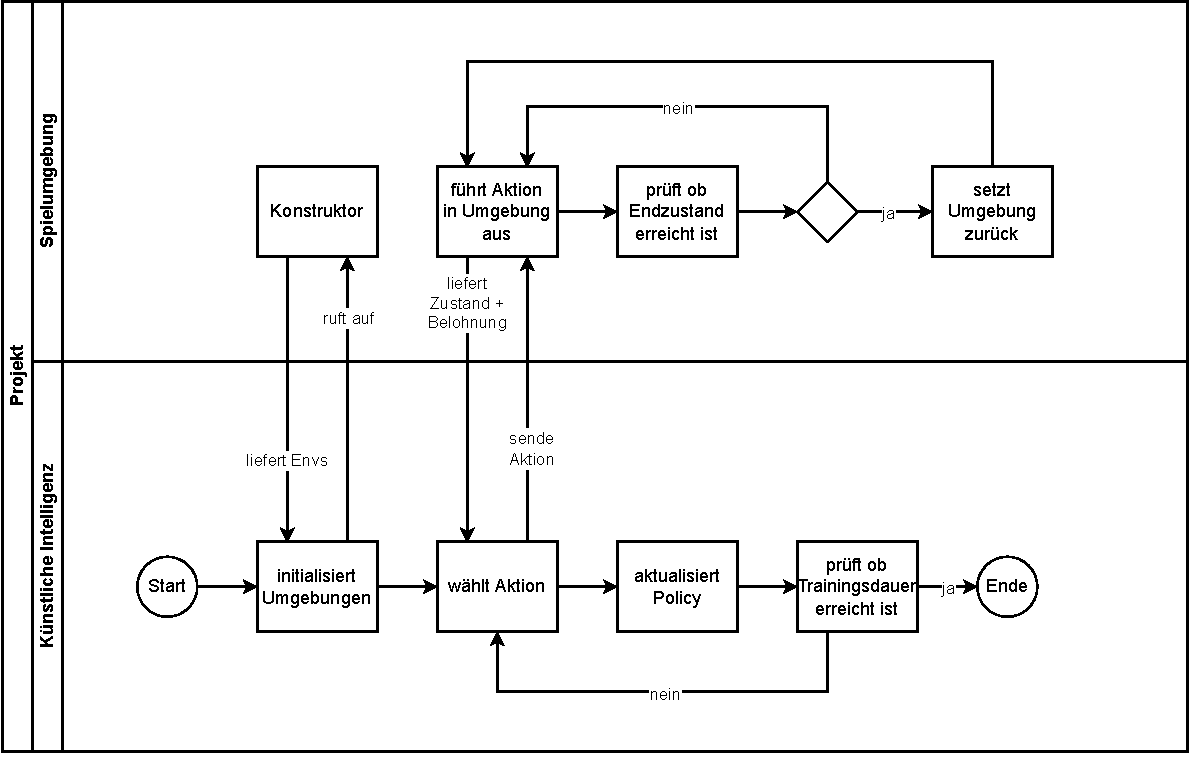
\includegraphics[width=1\textwidth]{Bilder/swimlane.drawio.pdf} 
	\caption[Swimlane-Diagramm des Trainingsprozesses der KI]{Swimlane-Diagramm des Trainingsprozesses der KI\\ Quelle: Eigene Darstellung}
\end{figure}	

Wie Abbildung 6 zeigt wird zunächst der Trainingsprozess angestoßen und die Umgebung wird initialisiert. Dazu wird der Konstruktor der Umgebung aufgerufen. Daraufhin wird eine Aktion von der KI ausgewählt und an die Umgebung weitergeleitet. Die Umgebung führt diese Aktion aus und prüft ob der Endzustand des Spiels erreicht wurde oder nicht. Wenn der Endzustand erreicht wurde, wird die Umgebung auf ihren Anfangszustand zurückgesetzt. Wenn der Endzustand nicht erreicht worden ist, wird der Prozess ohne Weiteres fortgesetzt. Daraufhin liefert die Umgebung der KI eine Belohnung [siehe Unterabschnitt 2.1.3] für den ausgeführten Schritt und den neuen Zustand der Umgebung nach Ausführung der Aktion.

Daraufhin aktualisiert die Künstliche Intelligenz ihr neuronales Netz mit der Policy und überprüft ob bereits genügend Zeit vergangen ist, um das Training zu beenden. Wenn die festgelegte Zeit vergangen ist wird das Training an dieser Stelle beendet. Wenn nicht wird die nächste Aktion gewählt und das Training wird fortgesetzt.

Dies ist lediglich eine vereinfachte Darstellung des Prozesses. In Wirklichkeit wird die Policy nicht nach jedem Schritt/jeder Aktion aktualisiert, sondern es wird erst eine festgelegte Menge an Aktions-Zustands-Paaren gesammelt. Dann wird das neuronale Netz mit dieser Gesamtmenge aktualisiert. Diese Aktions-Zustands-Paare ermöglichen es festzustellen, welche Aktionen in welchen Zuständen zu einem guten Ergebnis führten und welche nicht. Hierfür wird für jeden Zustand ein geschätzter Wert über seinen zukünftigen Nutzen erstellt. Dafür wird ein neuronales Netz, das sogenannte Value Network genutzt. Dieser geschätzte Nutzen wird mit dem tatsächlich erzielten Nutzen verglichen. Die Policy wird anschließend in Richtung vorteilhafter Zustände angepasst, die einen möglichst besseren tatsächlichen als erwarteten Nutzen aufweisen.
\subsubsection{Spielumgebung}
Die Abbildungen 7 und 8 zeigen den prinzipiellen Funktionsablauf in der Spielumgebung. Dabei wird am Anfang eine Aktion entgegengenommen und am Schluss der neue Zustand dieser Umgebung nach Ausführung der Aktion zurückgegeben:
\nopagebreak
\begin{figure}[H]
	\centering
	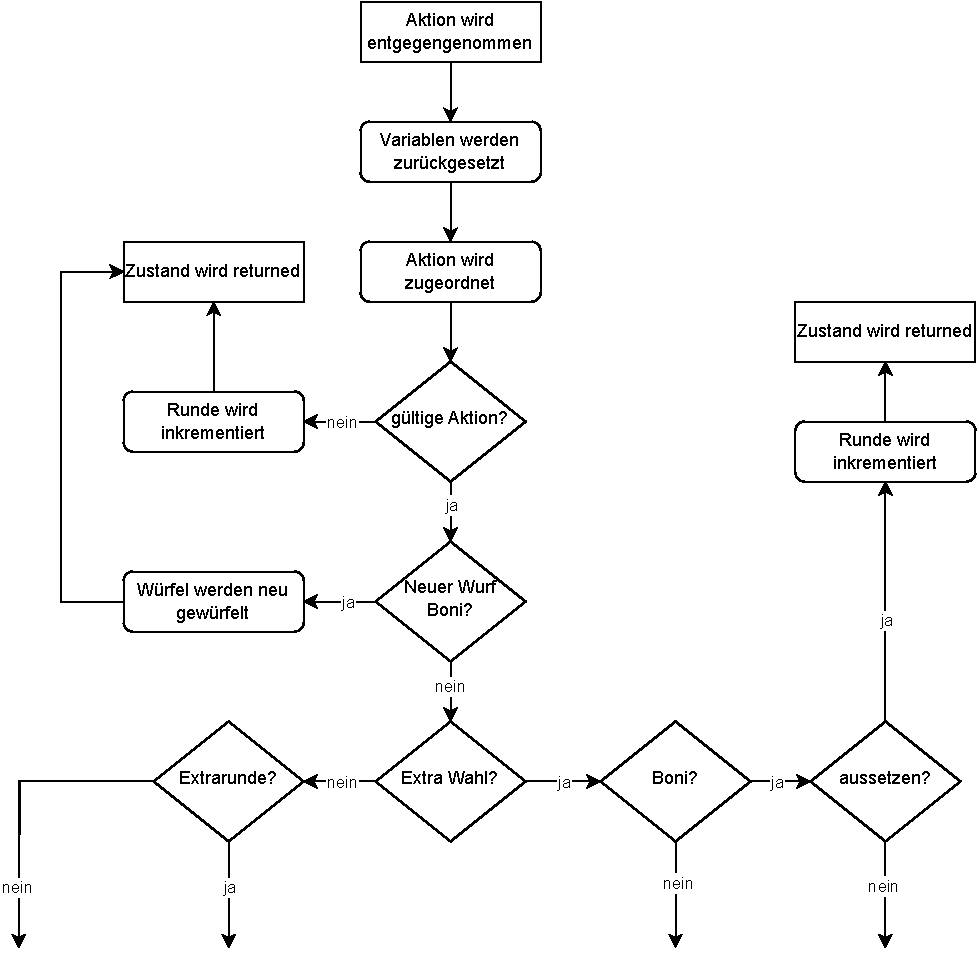
\includegraphics[width=0.9\textwidth]{Bilder/step3.drawio} 
	\caption[Ablauf-Diagramm der Schritt-Funktion 1]{Ablauf-Diagramm der Schritt Funktion 1\\ Quelle: Eigene Darstellung}
\end{figure}	

Wie Abbildung 7 zeigt wird der Vorgang durch eine Aktion angestoßen. Nach dem Anstoßen, werden die Variablen der Funktion zurückgesetzt, um einen klaren Schnitt zwischen vergangenen Aktionen und der aktuellen Aktion zu erzielen.

Anschließend wird die Aktion ihrem entsprechenden Ablauf zugeordnet. Es gibt Aktionen für Wahlen nach normalen Würfen, für Wahlen von Würfeln des Silbertablettes sowie für das Nutzen von Boni. Außerdem gibt es eine Aktion, die nur dann wählbar ist, wenn keine der anderen Aktionen gewählt werden kann. Dies ist die Aktion für ungültige Züge.

Ist die Aktion nicht gültig, wird die Runde inkrementiert und der Zustand der Umgebung zurückgegeben.

Wird die Neu Würfeln Boni verwendet, werden die gültigen Würfel neu geworfen und anschließend der Zustand zurückgegeben.

Ist beides nicht der Fall kommt es zu einer Auswahl zwischen den wesentlichen Aktionen der Umgebung. Es gibt sogenannte Extra-Wahlen. Diese spalten sich auf in Extra-Wahlen mit einem Extra-Wahl-Bonus und Wahlen vom Silbertablett eines Mitspielers.

Handelt es sich nicht um eine Extra-Wahl, so folgt eine Unterteilung in Extra-Runden und Normale-Runden. Bei Extra-Runden wird eine der Boni verwendet (in Abb. 8: Boni Wahl), die es erlauben eines der farbigen Felder direkt auszufüllen [siehe Unterabschnitt 2.1.1].

Handelt es sich nicht um eine Extra-Runde muss es sich in diesem Fall um eine Normale-Runde (in Abb. 8: Normale Wurf Wahl) nach einem gewöhnlichen Wurf handeln [siehe Abb. 2].

Handelt es sich um eine Extra-Wahl mit Boni (mit Extra-Wahl-Bonus), dann steht noch die Aktion "Passen" zur Wahl. Diese inkrementiert lediglich die Runde, sodass das Spiel weiter fortgesetzt werden kann. Dies spiegelt die Möglichkeit im Spiel wieder auf die Nutzung eines Extra-Wahl-Bonus zu verzichten.\\

\begin{figure}[H]
	\centering
	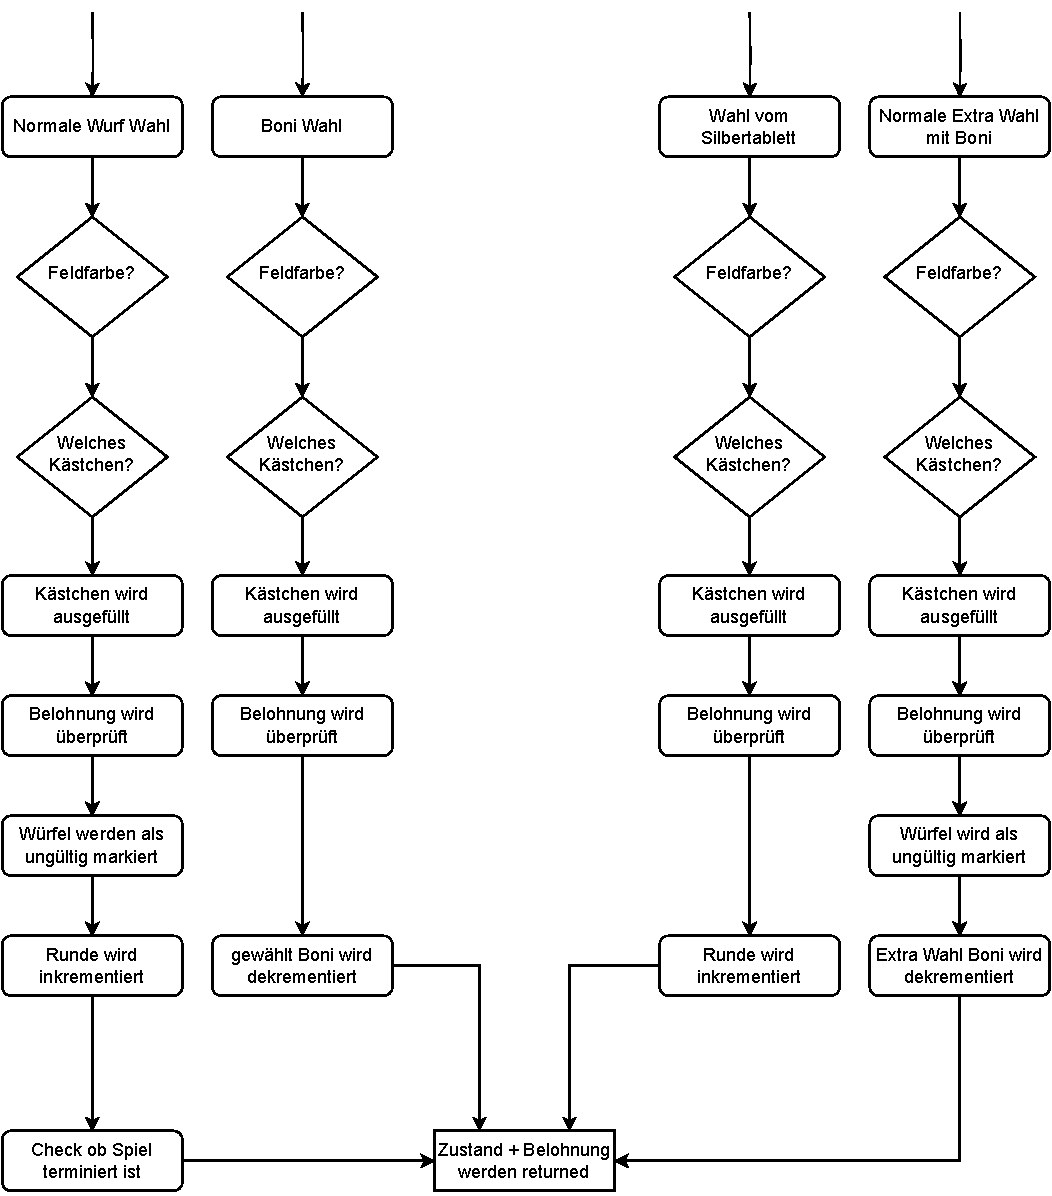
\includegraphics[width=0.9\textwidth]{Bilder/step2.drawio} 
	\caption[Ablauf-Diagramm der Schritt-Funktion 2]{Ablauf-Diagramm der Schritt Funktion 2\\ Quelle: Eigene Darstellung}
\end{figure}

Wie in Abbildung 8 dargestellt gestaltet sich der folgende Ablauf der Funktion relativ ähnlich bei allen vier Varianten. Es wird das Feld und das Kästchen ermittel, welches ausgefüllt werden soll und das entsprechende Kästchen wird anschließend ausgefüllt. Dann wird die Belohnung für diesen Schritt ermittelt.

Am Ende der Funktion unterscheiden sich die vier Varianten wieder. Bei einer Normalen-Runde nach einem normalen Wurf werden die entsprechenden Würfel als ungültig markiert [siehe Unterabschnitt 2.1.1] und die Runde wird inkrementiert. Außerdem prüft die Funktion bei dieser Variante am Ende, ob das Spiel terminiert ist oder nicht.

Beim Ausfüllen eines Feldes mittels eines Bonus (kein Extra-Wahl-Bonus) wird der entsprechende Bonus dekrementiert.

Bei der Extra-Wahl vom Silbertablett wird die Runde inkrementiert.

Bei der Extra-Wahl mittels Bonus wird der gewählte Würfel als ungültig markiert und der Extra-Wahl-Bonus dekrementiert.

Bei allen vier Varianten wird am Ende der Funktion der aktuelle Zustand der Umgebung sowie die erhaltene Belohnung für den Schritt zurückgegeben.

\subsubsection{Künstliche Intelligenz}
Abbildung 9 zeigt die wesentlichen Hyperparameter, die bei der Entwicklung der Künstlichen Intelligenz von Bedeutung sind:
\nopagebreak
\begin{figure}[H]
	\centering
	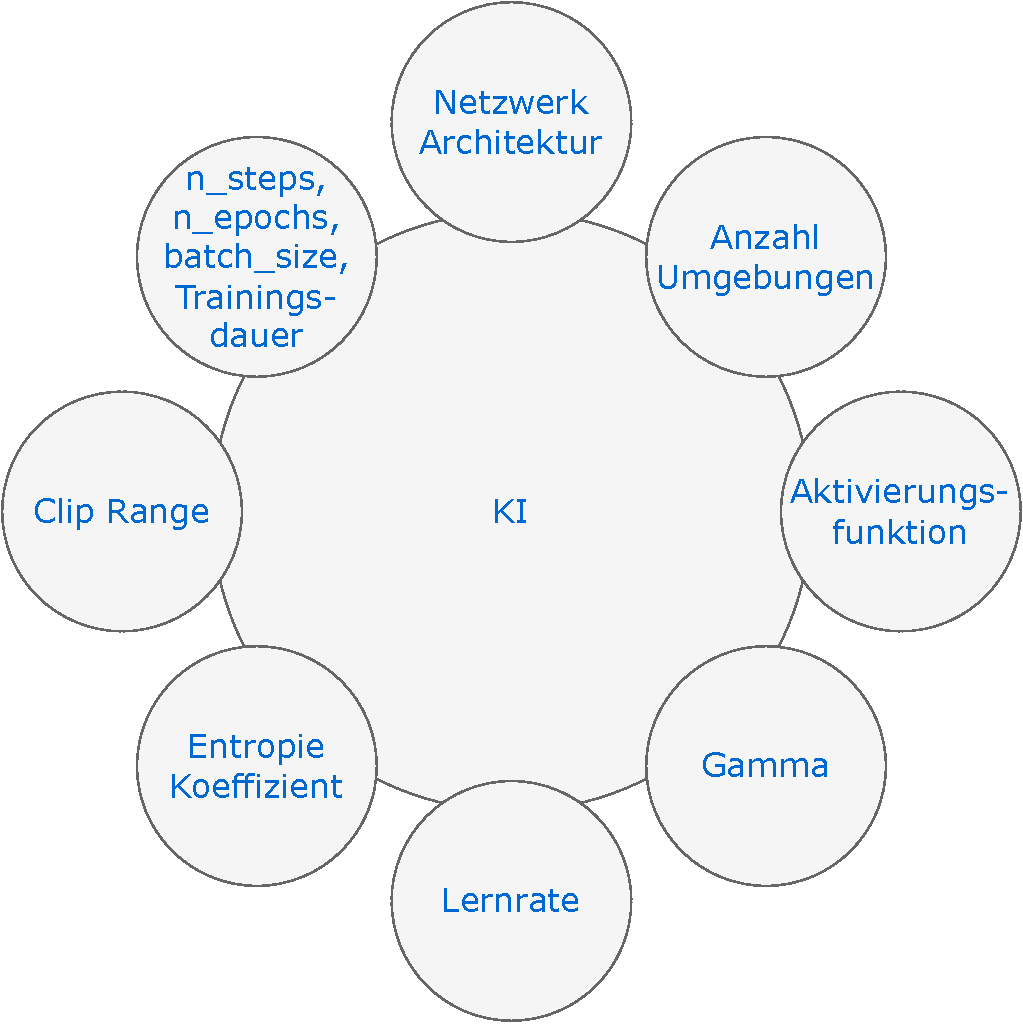
\includegraphics[width=0.6\textwidth]{Bilder/KI} 
	\caption[Wesentliche Hyperparameter der Künstlichen Intelligenz]{Wesentliche Hyperparameter der Künstlichen Intelligenz\\ Quelle: Eigene Darstellung}
\end{figure}

Die Künstliche Intelligenz basiert auf der MaskablePPO-Version von Stable Baselines 3 Contributing. Es sind Konfigurationen zu treffen, welche das Training beeinflussen und steuern. Diese Einstellungen werden Hyperparameter genannt. Hyperparameter legen die Ausprägung gewisser Steuerelemente des MaskablePPO-Algorithmus und ähnlicher Reinforcement-Learning-Algorithmen fest.

Die wichtigsten Hyperparameter für das Projekt sind folgende [siehe Abb. 9]:

\begin{itemize} 
\item Netzwerkarchitektur: Legt die Anzahl der Schichten des neuronale Netzes fest, Dieses Netz wird zur Abbildung der Policy verwendet. Außerdem legt die Netzwerkarchitektur fest, wie viele Neuronen es pro Schicht gibt [siehe Unterabschnitt 2.1.4]. Die Netzwerkarchitektur ist so zu bestimmen, dass die Künstliche Intelligenz im Stande ist, die Komplexität der Problemstellung zu erfassen und gleichzeitig zu gewährleisten, dass die Trainingsdauer und die Systemauslastung dadurch nicht zu hoch steigen. Außerdem sollte es nicht zu einer Überanpassung an die Trainingsdaten kommen. Da es sich bei dem neuronalen Netz um ein Multilayer Perceptron handelt, sind alle Neuronen einer Schicht mit allen der vorherigen und folgenden Schicht verbunden [siehe Unterabschnitt 2.1.4]. Dies führt dazu, dass die Rechenleistung für das Updaten der Gewichte der Policy exponentiell steigt, je komplexer das neuronale Netz wird. Dies führt zu einer gesteigerten Trainingsdauer und Systemauslastung. Außerdem tendieren zu komplexe Neuronale Netze dazu, sich stark an die Trainingsdaten anzupassen, was zu Überanpassung führen kann. Zu komplexe Netze generalisieren tendenziell schlechter auf neue Datensätze, die sich stark von den Trainingsdaten unterscheiden.

\item Anzahl der Umgebungen: Eine erhöhte Anzahl an Trainingsumgebungen ermöglicht es, besonders bei Nutzung von CUDA (GPU), parallel Daten aus mehreren Umgebungen zu sammeln und zu verarbeiten. Dies erhöht die Trainingsgeschwindigkeit, da ein erheblicher Teil der Trainingsdauer in diesem Projekt davon abhängt, wie schnell die nötigen Trainingsdaten aus den Umgebungen generiert werden können. Außerdem erhöht die Nutzung von CUDA die Geschwindigkeit von Policy Updates enorm, da viele der Berechnungen im neuronalen Netz parallel abgearbeitet werden können. Allerdings erhöht die Anzahl der Umgebungen die RAM Auslastung enorm und die CPU Auslastung mittelmäßig stark, was dazu führt, dass es ineffizient wäre auf dem verwendeten System (Nvidia Geforce GTX 1070, Intel i5 8600k, 16GB RAM) deutlich mehr als 32 Umgebungen zu betreiben.

\item Aktivierungsfunktion: Legt zusammen mit den Gewichtungen der Neuronen fest, wann und wie stark diese ihre Signale an die folgenden Neuronen weiterleiten. Im Projekt wird vor allem die ReLU-Funktion verwendet, da diese standardmäßig vom Algorithmus verwendet wird und im allgemeinen sowie spezifisch in diesem Projekt gute Ergebnisse erzielt. Die Formel der ReLU-Funktion lautet: f(x) = max(0,x). Die ReLU-Funktion gibt, wenn der Wert kleiner als Null ist, Null zurück und ansonsten den Wert selbst \cite{schmidt-hieber_nonparametric_2020}.
\end{itemize} 

Abbildung 10 zeigt den Graphen der ReLU-Funktion:
\nopagebreak
\begin{figure}[H]
	\centering
	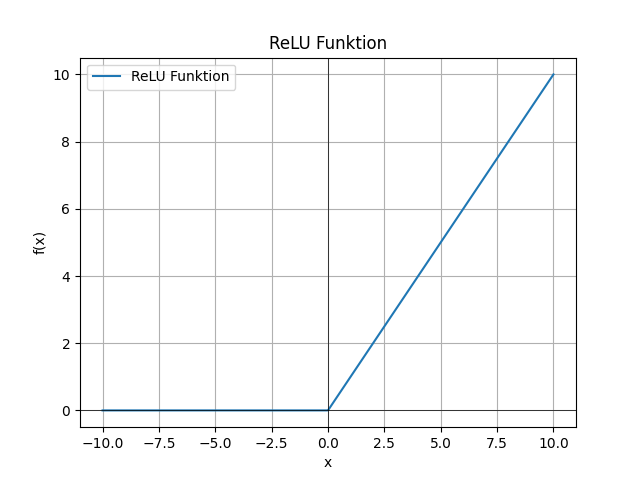
\includegraphics[width=0.7\textwidth]{Bilder/ReLU} 
	\caption[Graph der ReLU-Funktion]{Graph der ReLU-Funktion\\ Quelle: Eigene Darstellung}
\end{figure}

\begin{itemize} 
\item Gamma: Legt fest, wie stark zukünftige Belohnungen wertgeschätzt werden. Es fungiert als eine Art Multiplikator. Potenzielle Belohnungen werden pro Spielschritt, den sie in der Zukunft entfernt liegen würden, mit Gamma multipliziert. Gamma ist so zu wählen, dass das Modell lernt, die bestmöglichen Aktionen zu wählen, um insgesamt das beste Ergebnis zu erzielen. Zu hohe Werte von Gamma können dazu führen, dass kurzzeitige Belohnungen vernachlässigt werden, was zu einem schlechteren Gesamtergebnis führen kann, wenn diese von besonderer Bedeutung sind. Zu niedrige Werte von Gamma können wiederum dazu führen, dass der Agent nicht zukunftsorientiert handelt und somit kein gutes Gesamtergebnis erzielt, da er sich hauptsächlich auf kurzfristige Belohnungen konzentriert, anstatt in die Zukunft zu schauen und dieser Wert zuzumessen. In diesem Projekt bewegt sich der Wert von Gamma im Allgemeinen in einem Bereich zwischen 0.5 und 1.

\item Lernrate: Bestimmt, wie stark Updates des neuronalen Netzes und seiner Gewichtungen pro Updateschritt ausfallen. Zu große Werte für die Lernrate können zu einem instabilen Training führen, da die Updates somit stark vom Trainingsdatensatz abhängen. Zu niedrige Werte führen wiederum zu einer Erhöhung der benötigten Trainingsdaten und Trainingsdauer. Der Wert für die Lernrate bewegt sich im Projekt üblicherweise zwischen Werten von 0.0003 bis zu 0.0003x32.

\item Entropie-Koeffizient: Bestimmt das Maß an Exploration des Modells. Je höher der Entropie-Koeffizient ist desto stärker Belohnt das Modell neue beziehungsweise bisher wenig erkundete Aktionen oder Zustände. Ein zu hoher Wert führt dazu, dass das Modell nicht lernt bereits funktionierende Taktiken ausreichend zu verfestigen. Ein zu niedriger Wert führt dazu, dass das Modell sich relativ schnell auf eine bisher vergleichsweise gut funktionierende Strategie festlegt und diese verfestigt. Der Entropie-Koeffizient bewegt sich innerhalb des Projektes meist zwischen Werten von 0.05 und 0.3, wobei sich ein Wert um die 0.1 als stabil und effizient herausgestellt hat.

\item Clip-Range: Die Clip-Range ist spezifisch für den PPO-Algorithmus [siehe Unterabschnitt 2.1.5]. Sie legt fest wie stark Policy Updates sein dürfen und ab welchem Schwellwert die Updates abgeschnitten werden. Abschneiden heißt, dass die Updates zwar durchgeführt werden, allerdings darf die Policy nach dem Update nur maximal um einen bestimmten Wert von der vorherigen abweichen. Die standardmäßige Clip-Range beläuft sich auf 0.2. Innerhalb des Projektes werden auch andere Werte getestet.

\item nSteps: Legt fest, wie viele Aktions-Zustands-Paare gesammelt werden, bevor ein Update des neuronales Netzes erfolgt.

\item nEpochs: Legt fest wie oft dasselbe Datenpaket von nSteps für das Training benutzt wird bevor es verworfen wird. Je öfter man es verwendet, desto weniger Daten braucht man und desto schneller verläuft das Training. Allerdings sollte der selbe Datensatz nicht zu häufig verwendet werden, um Überanpassung zu vermeiden. nEpochs hat im Rahmen des Projektes üblicherweise einen Wert zwischen 5 und 11.

\item Batch Size: Das Datenpaket von nSteps wird vor der Verwendung für das Updaten des neuronalen Netzes in kleinere Datenpakete, die sogenannten Batches, zerlegt. Daraufhin werden Updates mit jedem dieser Batches durchgeführt. Die Aufteilung erfolgt per Zufall, daher ist mit hoher Wahrscheinlichkeit keines der Datenpakete (Batches) wie das andere, selbst wenn dasselbe Gesamtdatenpaket durch ein hohes nEpochs viele male verwendet wird. Batch Size legt fest wie groß diese kleineren Datenpakete (Batches) sind.

\item 
Trainingsdauer: Die Trainingsdauer legt fest wie lange trainiert wird. Die Implementierung von Stable Baselines [siehe Kapitel 2.2.2] verwendet standardmäßig Timesteps zur Messung von Zeit. Eine Timestep ist ein ausgeführter Schritt beziehungsweise eine ausgeführte Aktion in einer Umgebung. Die Timesteps von mehreren parallel laufenden Umgebungen werden aufsummiert, somit kommt es nicht zu vermehrtem Training alleine durch Erhöhung der Umgebungsanzahl bei gleichbleibender Trainingsdauer in Timesteps.
\end{itemize}